\Chapter{Roadwater}{Glyn Court}

It was in Higher Roadwater, which lies at the geographical centre of the parish, that for more than a hundred years my family made their home. They lived in a spacious William and Mary farmhouse, with a garden and orchard running down to the little stream which form the western boundary of the parish of Nettlecombe. If spaciousness calls up a vision of landed wealth and patrician ease, I must confess, though not without a certain pride, that none of the Courts has ever gained a superfluity of wealth, ease or leisure. Yet their modest means and stationary position have given them interest, for they have been concerned in the life of this parish, in many different capacities, for most of two centuries, and their lives illustrate the movements which have altered or sustained, our society for much of that time, moreover, having been unusually aware of the processes of change, they have consciously tried to preserve the form and spirit of the good traditions of former times, the memory of the worthies of the parish, and also a host of treasure objects which recalled to them the vanished lineaments of those whom they had loved and lost in the golden days of their youth. The associations gathering round these treasures were kept alive and cherished, through several generations, by word of mouth, and it has been my pleasure - though one tinged at times with sorrow - to capture and record many of them in this book.

One who was devoted to the memory of an older time used to dwell lovingly on those haunting lines of Longfellow:

\begin{quote}
And the friendships old and the early loves \\
Come back with a Sabbath sound as of doves \\
In quiet neighbourhoods... \\
And the thoughts of youth are long, long thoughts;
\end{quote}

and others since his day have looked back longingly to that vanished world and felt the tears rise within them with the yearning for that tranquil land of eternal Sunday which they have never known.

\Flourish 

The old homesteads of Roadwater, in the early days of Queen Victoria’s reign must have looked very much like those of Acadie so lovingly described in ’Evangeline’:

\begin{quote}
Strongly built were the houses, with frames of oak and of hemlock, \\
Thatched were the roofs, with dormer windows, and gables projecting. \\
There in the tranquil evenings of summer, brightly the sunset \\
Lighted the village street with mysterious splendour, and roofed each  \\
Peasant’s cottage with golden thatch and. emblazoned its windows.
\end{quote}

One suspects, however, that visitors would have appreciated this rustic splendour more keenly than some of the people who dwelt there. 

Some of the cottagers in those good old days could, if they had been of the complaining sort, have told you more about the bad side - the grinding poverty, the overcrowding, the infected water, the diphtheria and consumption, the chronic \quotemark{rheumatics}, the workhouse. But for those with the leisure to look around, and the eye to see beauty, the landscape had attained its perfection after long generations of maturing. In the village the speculative builder had not arrived, mean little bungalows and open-plan development had not been dreamed of even in nightmares, and the farmhouses and cottages were still being built with local materials in a living local tradition.

Unfortunately, no artist has left a record of the lineaments of Roadwater in those days, but I should like to try, with the help of family reminiscences and the tithe map, to reconstruct its appearance a hundred and more years ago.

\begin{figure}[p]
     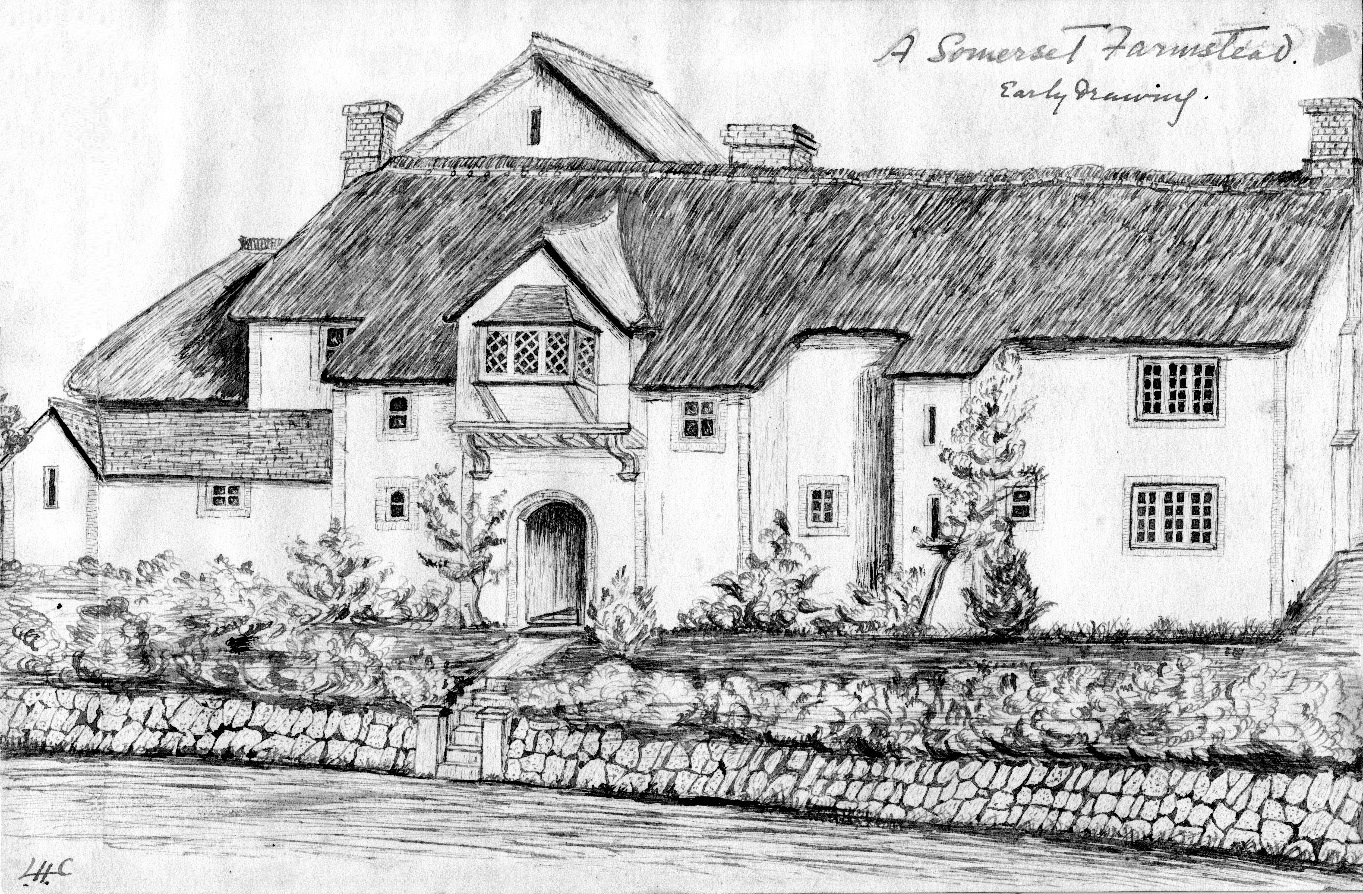
\includegraphics[width=1\textwidth]{figures/Glasses}
     \caption{Glasses, a seventeenth century farmhouse, Roadwater}
     \label{fig:Glasses}
\end{figure}


We approach it from Washford, along the narrow road past Roughmoor, ankle-deep in mud or dust according to the season. At the entrance to the village, where the side-road comes in from Clitsome - it does not connect directly with Beggearnhuish - the open brook flowing down from Roadwater Farm and past the picturesque cottage on the corner, forms a ford, with a footbridge; but the first substantial building in the village is the prosperous Roadwater Inn, and there is little else, apart from Roadwater Farm and Yea Farm, until we come to Manor Mills. Rounding the corner, we see on the right, where the mission church has since been built, two cottages and a lime kiln; but on the left there is no building until we reach the four Day Mead Cottages, on the site of the Village Hall and close to the corn mill. (Day's Meadow itself stretched considerably further up the valley than the present recreation ground, but even then it was used for the village revels and entertainments.)

The mill leat, which is taken off from the Luxborough stream a good way up and flows through gardens and out by the village shops, here runs open by the right-hand side of the road and then under into the mill.

There is a building up on Knap, the New Inn, kept by Robert Flueilen, a burly man with a determined expression. He gains additional income from tailoring, though in a village community most of his work consists of repairs and alterations, cutting down Stephen's \quotemark{jackett} to fit Albert and so on.

Behind the village shop is a chandlery, which needs no notice to announce its business: the aroma of tallow is its own advertisement.

\begin{figure}[p]
     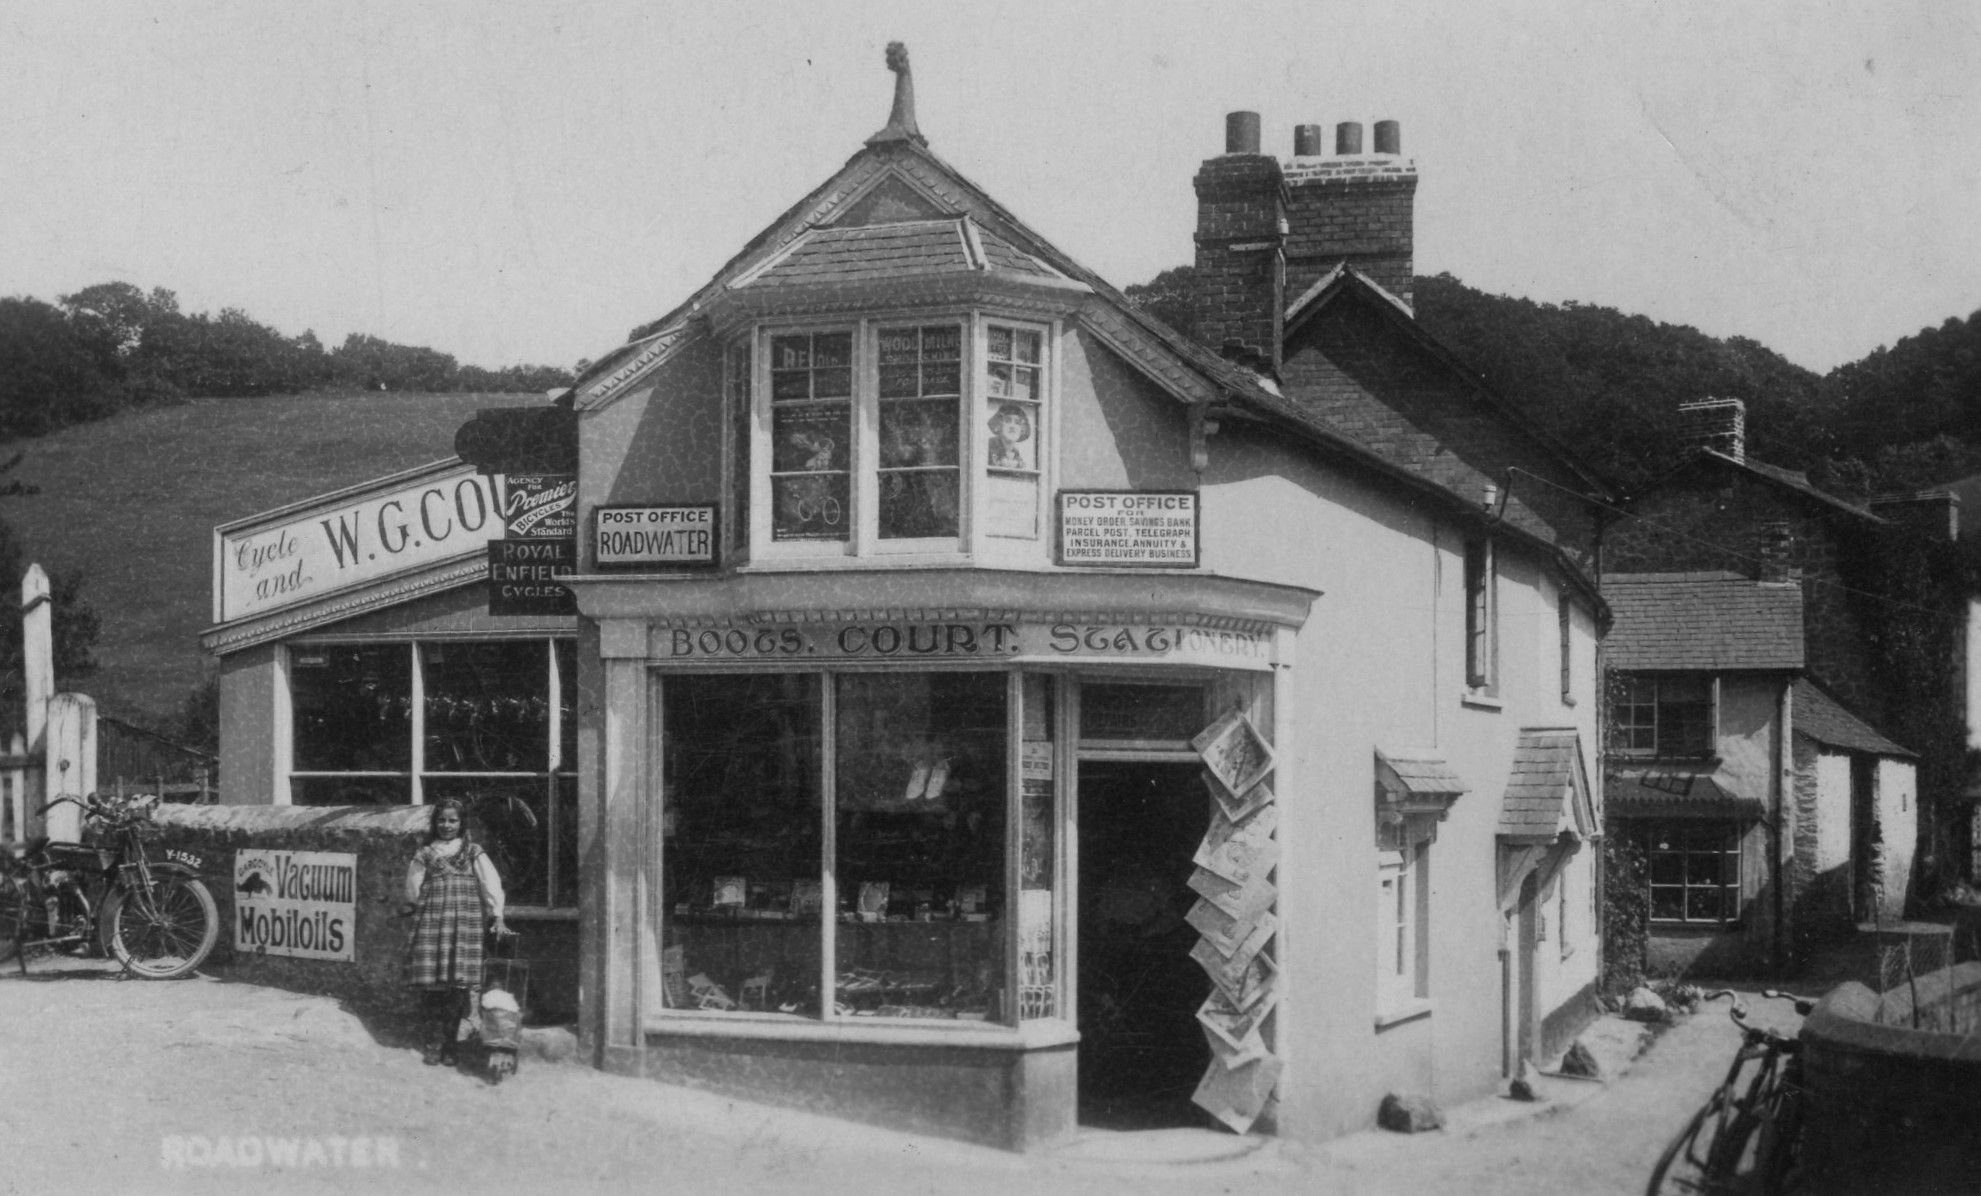
\includegraphics[width=1\textwidth]{figures/bridgeVillageShop}
     \caption{The Bridge Village Shop, Roadwater}
     \label{fig:BridgeShop}
\end{figure}

Beyond here the road dips slightly to the ford through the river, though on the right a stone footbridge is provided by the dipping place. There are signs of new building, however, and on the left the railway company are putting up a house for their Roadwater agent, and they are also preparing to raise the level of the road, roof over the stream and provide stone steps down to a new dipping place. In the garden of the house stand two gigantic poplar trees, and on the right of the road arc two cottages with lilac trees.

Here the road to Wood Advent branches off, running alongside an orchard. There are no buildings on the left of Proud Street (soon to be called station Road, but still taking its name from the Prowsc family) and Oatway House has a fine view down the valley. Beyond the ford at the bottom of Harper's, and over on the right, under the bank below Coachroad, is a blademill, powered by a leat coming down through the fields from Hayne, and run by George Edbrooke, who, in addition to the usual blacksmith's work, had made the iron gates for Old Cleeve Church and also specialises in scythes, billhooks, ploughshare and cutting edges of many kinds. But though the leat comes down from Hayne, there is no road up the valley, and the cottages at Traphole and Hayne are connected with Leighland, not Roadwater.

On the high, rough area known as Scrubbit, the barns are still thatched and in use, and the children play under a fine walnut tree fifteen feet around; while on Hill Close there stands a magnificent oak tree six feet in diameter.

The road up towards Luxborough leads past the Bible Christian chapel, built in 1842 on the only ground available, and set right into the bank of Scrubbit; already suffering from damp, of course, but still in good shape, even if too small for the constantly increasing congregations from the periodic revivals. From here the church path to Leighland and Stamborough leads up over the hill, past the allotments looking down on the Valiant Soldier, past the sawpits and the mounds of charcoal-burners. Nearby the rackfield, where the cloth from the fulling mills down at Vale is laid out to dry. And indeed, the number of mills in this valley is quite extraordinary, for the little stream without even a name, drives no fewer than twelve, from Luxborough and Leigh, through Roadwater and Washford right down to Watchet.

I mentioned earlier the poverty and overcrowding within the picturesque cottages, and social historian such as Ernest Martin, Walter Crotch and F. E.  Green have written movingly of the inhuman conditions so patiently endured. But to complete this survey I will describe in some detail the cottage best known to me from childhood, that in which our branch of the family lived for a hundred years:

\begin{center}
A cottage by the Brendon brook \\
With many a diamond casement pane \\
That looked out on a winding lane:
\end{quote}

those lines by one who was born in \quotemark{Oatway} in 1870 briefly describe the exterior, but they give no idea of the homely charm that greeted you when you stepped over the threshold.

\quotemark{Cottage} is rather a misnomer. It was spacious, and could have held two families. A yeoman of Nettlecombe, William Oatway, had built it as a dower house for his daughter in 1700, and the date and his initials could clearly be seen worked in the plaster high up on the front wall under the thatched eaves. In front, the vegetable garden ran down to the river, where there were steps for dipping water; behind, a cobbled court led up to a stable and an orchard with beehives, and on to an area of high rough ground known as Scrubbet, where the ruins of a barn witnessed to the former farming  history of the property. The house was built to a plan very frequently used in West Somerset; a porch at one front led into a passage which ran right through to the back court, and one door on the right and another on the left gave entrance to two separate dwellings. All visitors come in by the back door, as the front door gave only on to the garden. Once you crossed the threshold and took one step down you found yourself in a very large red-tiled kitchen with a low ceiling and oaken beams. The room was lit by two leaded casements and, at night, by a paraffin lamp placed on a table under a white enamelled dome. The table, which occupied all the centre of the kitchen, was large enough to seat twelve, and at Christmastide it often did. Against one wall stood the massive grandfather clock, which it had been Grandfather’s care to recover on restoring the family fortunes: the face was decorated with an inscrutably smiling sun, and marked the seasons, and it proclaimed itself the work of \quotemark{John How, Watchet}. Next to the clock stood a glass-fronted double bookcase which was not locked but kept closed with a late Victorian curiosity: a biscuit-tin shaped like a book and bearing the illuminated words and music of \quotemark{Good King Wenceslas}. The bookcase itself - I am of course speaking of the time of my boyhood, not of Victorian days - was filled with biographies and studies of history, especially of Methodism: Southey’s Life of Wesley; \quotemark{Gladstone; A Popular Biography}; \quotemark{The King's Son: The Life of Billy Bray}; \quotemark{The Romance of a Country Circuit}; Lord Roseberry's \quotemark{Napoleon, the Last Phase}; \quotemark{The Voyage of the Medusa} - the variety and number were, for the time and place, extraordinary and were reflected in Grandfather's well-furnished mind and his ready command of speech on formal and informal occasions alike.

The kitchen range was, I surmise, a late Victorian improvement, with a high fire box for convenience and a capacious oven on the left, while the right-hand side contained a tank in which water could be heated and drawn off through a brass tap. To the right of the fireplace there always stood Grandfather's hard upright armchair; to the left a high partition had been erected to keep off the draught, and this was provided with a long seat, so that the focal point of the room was, as the word implies, the fireplace. On the walls were various pictures of which I shall speak later.

From the left-hand corner of the kitchen a short flight of stairs, lit by a glazed arrow-slit on the outside wall, led up to the bedrooms - or rather, the bedroom, which had been divided into three by partitions. The floors were, need I say, the bare planking.

From the far side of the kitchen a short passage led to a tiny scullery and larder and also to the parlour, which contained a table covered with a red plush cloth and bearing a stuffed squirrel in a glass case. A side table displayed an elegent mid-Victorian rosewood writing cabinet presented to Grandfather by admirers.

A side-door from this room gave on to the village street, but it was seldom used. The parlour, likewise, was a \quotemark{best} room, a Sunday room, and it was used just as rarely, even on Christmas or Boxing Days, unless jinks of the younger generations in the kitchen became too elevated for grave and reverend age.

\Flourish

One observation has continually been made to me in conversing with men and women of an earlier generation: in villages such as Roadwater there was no prosperity, but oppressive poverty and privation; yet there was happiness. Having little, they desired little; they had few possessions but held firmly to certain fixed and incontrovertible truths; and they surely have much to tell us for our good, if we will listen, in our modern discontent.
